\documentclass[11pt,a4paper]{article}
\usepackage[T1]{fontenc}
\usepackage[latin1]{inputenc}
\usepackage{lmodern}
\usepackage{a4wide}
\usepackage[dvips]{graphicx}

\usepackage{float}

\usepackage[
pdfauthor={ACE Project Team},
pdftitle={User Manual},
pdfcreator={pdftex},
]{hyperref}

\usepackage{sectsty}
\allsectionsfont{\sffamily}

\usepackage{fancyheadings} 
\pagestyle{fancy} 
\lhead{\textsf{\textbf{ACE} \\ \small{a collaborative editor}}}
\chead{}
\rhead{
\parbox[c]{3cm}{
\includegraphics[height=0.875cm,width=3cm]{../../images/logo_BFH.eps}}
\parbox[c]{2.2cm}
{\tiny{\textsf{Berner Fachhochschule \\
Hochschule f�r \\
Technik und Informatik}}}}
\lfoot{}
\cfoot{\textsf{\thepage}}
\rfoot{}
\setlength{\headrulewidth}{0.6pt}
\setlength{\footrulewidth}{0.6pt}
\setlength{\topmargin}{-50pt}
\addtolength{\headheight}{50pt}

\usepackage{colortbl}

\newcommand{\headercol}[2]{\multicolumn{1}{|>{\bfseries\columncolor[gray]{0.82}}p{#1}|}{\textsf{#2}}}
\newcommand{\ace}[0]{\emph{ACE }}



\begin{document}

\setlength{\parindent}{0pt}

\begin{titlepage}
\thispagestyle{empty}
  
\includegraphics[height=1.5in]{../images/pix.eps}

  \begin{center}

    {\fontsize{40}{45} \textbf{\textsf{ACE}}} \\
    \textsf{a collaborative editor} \\
        
    \vspace{36pt}
        
    {\huge{\textbf{\textsf{}}}} \\

    \vspace{36pt}

	\textsf{Berne University of Applied Sciences} \\
    \textsf{School of Engineering and Information Technology} \\
    
  \end{center}

  \vfill
  
  \begin{tabular}{ll}
   \hline

   \\

   \multicolumn{1}{>{\bfseries}p{1.5in}}{\textsf{Date:}} &
   \multicolumn{1}{>{}p{4.3in}}{\textsf{08.11.2005}}          \\
   
   \\
   
   \multicolumn{1}{>{\bfseries}p{1.5in}}{\textsf{Version:}}     &   
   \multicolumn{1}{>{}p{4.3in}}{\textsf{0.1}}                 \\

   \\
   
   \multicolumn{1}{>{\bfseries}p{1.5in}}{\textsf{Projectteam:}}                 &
   \multicolumn{1}{>{}p{4.3in}}{\textsf{Mark Bigler (biglm2@hta-bi.bfh.ch)}}  \\
   \multicolumn{1}{>{\bfseries}p{1.5in}}{}                                      &
   \multicolumn{1}{>{}p{4.3in}}{\textsf{Simon Raess (rasss@hta-bi.bfh.ch)}}    \\
   \multicolumn{1}{>{\bfseries}p{1.5in}}{}                                      &
   \multicolumn{1}{>{}p{4.3in}}{\textsf{Lukas Zbinden (zbinl@hta-bi.bfh.ch)}} \\   
   
   \\
   
   \multicolumn{1}{>{\bfseries}p{1.5in}}{\textsf{Receivers:}}                       &
   \multicolumn{1}{>{}p{4.3in}}{\textsf{Jean-Paul Dubois (doj@hta-bi.bfh.ch)}}       \\
   \multicolumn{1}{>{\bfseries}p{1.5in}}{}                                          &
   \multicolumn{1}{>{}p{4.3in}}{\textsf{Claude Fuhrer (frc@hta-bi.bfh.ch)}}       \\

   \\
   
   \multicolumn{1}{>{\bfseries}p{1.5in}}{\textsf{Location:}}               &   
   \multicolumn{1}{>{}p{4.3in}}{\textsf{Subversion Repository}} \\

   \\  
   
   \hline
  \end{tabular}

\end{titlepage}


\tableofcontents






\newpage
% 1. INTRO
\section{Introduction}

The \emph{User Manual} contains information on how use the application ACE. Further, information about the installation is given.






% 2. INSTALLATION
\section{Installation}
To run ACE, you need the following components installed on your local machine:
\begin{itemize}
 \item Java Runtime Environment (JRE) - 1.4.2 or higher \\
 Download: \href{http://java.sun.com/j2se/1.5.0/download.jsp}{http://java.sun.com/j2se/1.5.0/download.jsp}
 \item Bonjour (Only for Windows) \\
 Download: \href{http://www.apple.com/downloads/macosx/apple/bonjourforwindows.html}{http://www.apple.com/downloads/macosx/apple/bonjourforwindows.html}
\end{itemize}

Downloads for Linux and other Operating Systems:

\begin{itemize}
 \item Bonjour \\
 Download: \href{http://developer.apple.com/networking/bonjour/download}{http://developer.apple.com/networking/bonjour/download}
 \item Apache Ant \\
 Download: \href{http://ant.apache.org/}{http://ant.apache.org/}
 \item Maven Ant Task \\
 Download: \href{http://maven.apache.org/}{http://maven.apache.org/}
\end{itemize}

% 2.1 MAC
\subsection{Macintosh}
Mac OS X users do not have to install any other software beside ACE itself. The current version of ACE can be downloaded at \href{http://ace.iserver.ch}{http://ace.iserver.ch}.

% 2.2 LINUX
\subsection{Linux and other Operation Systems}
Chances are high that if there is a Java Runtime Environment for your operating system, ACE will work. Unfortunately, there is no installer for Bonjour on Linux, Solaris, ... That means, you have to build Bonjour from source. In the following instructions, replace os=linux with your operating system. Check the Makefile in \texttt{mDNSPosix/Makefile} for supported operating systems.


\begin{enumerate}
\item download the source code
\item unpack the downloaded tar.gz to a location of your choice
\item go to the subdirectory mDNSPosix
\item in the Makefile, adjust the variable \textit{JDK} to point to the correct JDK location
\item type make \texttt{os=linux} to build the mDNSResponder
\item as root user, type \texttt{make os=linux install} to install the mDNSResponder daemon
\item now, the daemon needs to be started by running the startup script \texttt{/etc/init.d/mdns start} as root
\end{enumerate}

Further, you have to build a shared library in order that Bonjour for Java works:

\begin{itemize}
\item in the directory mDNSPosix type \texttt{make os=linux Java}
\item as root, copy the file \texttt{libjdns\_sd.so} from \texttt{build/prod} to somewhere into the Java library path (system property java.library.path)
\end{itemize}

Next you can download the current version of ACE for other platforms from \href{http://ace.iserver.ch}{http://ace.iserver.ch}. To run ACE, type \texttt{ant run} in the top-level directory. Note: you need Apache Ant and Maven Ant Task installed in that case.

% 2.3 WINDOWS
\subsection{Windows}
Windows users have to install a Java Runtime Environment (JRE) - 1.4.2 or higher. Further, Bonjour for Windows has to be downloaded and installed. If you have iTunes on your computer, Bonjour is already installed. The ACE installer guides your through the installation and warns you, if Bonjour is not installed. \\
 \\
The current version of ACE can be downloaded at \href{http://ace.iserver.ch}{http://ace.iserver.ch}.





\newpage
% 3. OVERVIEW
\section{Overview}
ACE 
\begin{figure}[htbp]
\begin{center}
  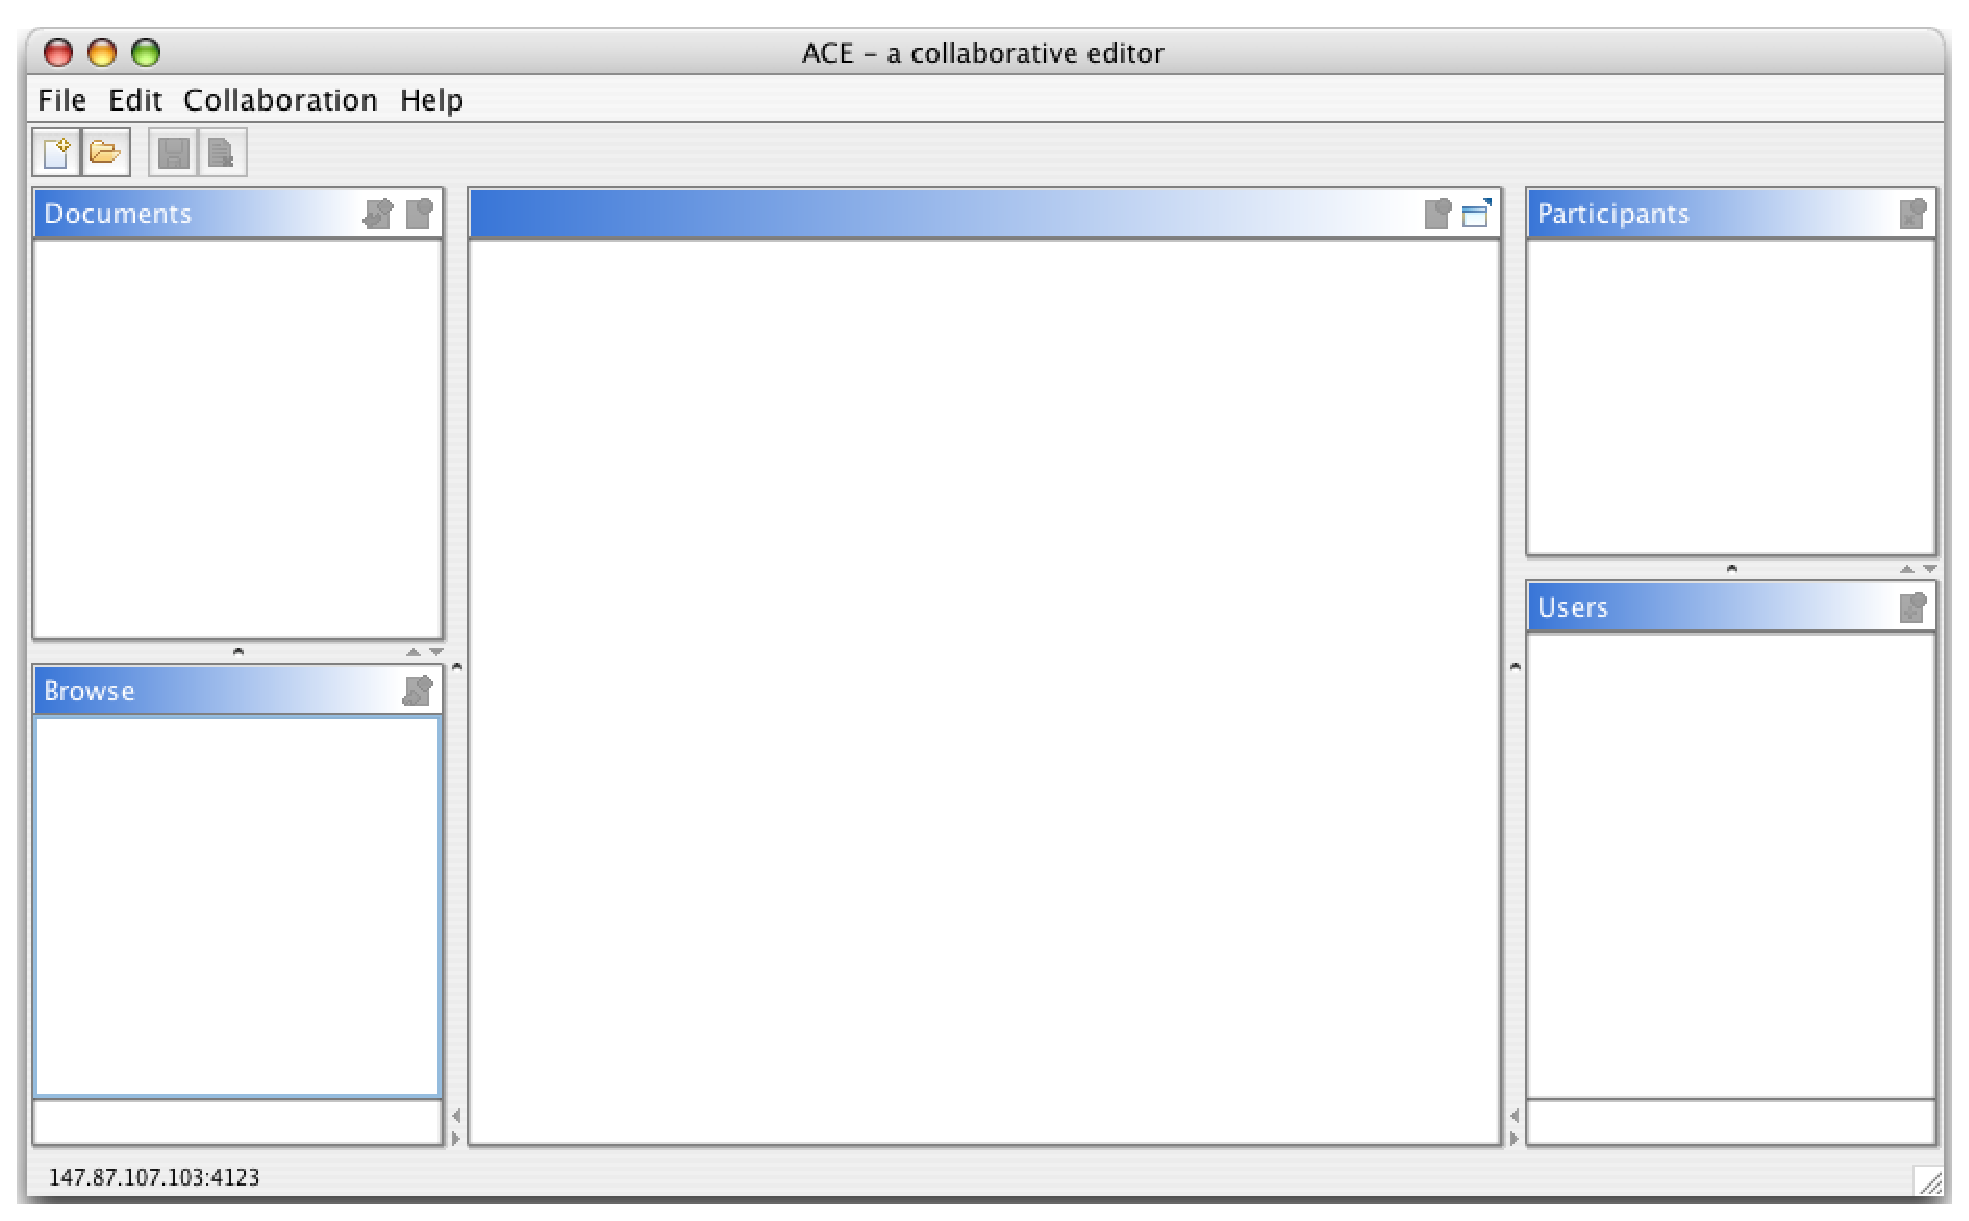
\includegraphics[height=30pt, width=30pt]{../images/usermanual/ace_overview.bmp.eps}
\caption{Browse View Filtering}
\label{default}
\end{center}
\end{figure}


% 3.1 MENUS
\subsection{Menus}
\begin{itemize}
\item File Menu
\item Edit Menu
\item Collaboration Menu
\item Help Menu
\end{itemize}

% 3.2 EDITOR
\subsection{Editor}
- Switch to FullScreen
- (Bild: %editor_overview)
- (Bild: %editor_collab_01)
- (Bild: %editor_collab_02)

% 3.3 VIEWS
\subsection{Views}
- alle views haben toolbars

% 3.3.1 DOCUMENT VIEW
\subsubsection{Document View}
\begin{figure}[htbp]
\begin{center}
  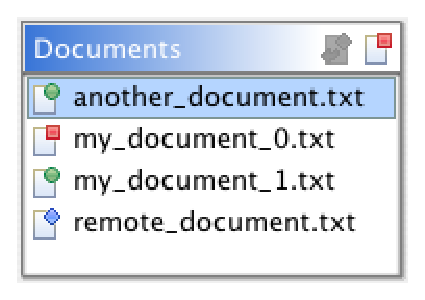
\includegraphics[height=30pt, width=30pt]{../images/usermanual/dview_overview.bmp.eps}
\caption{Document View}
\label{default}
\end{center}
\end{figure}

The \textit{Document View} shows all your currently open documents. Basically there are two different document types. \textit{Local documents} are documents on your local machine. ACE provides you the standard editor functionalities as create new, open, save and close local documents. Further, you can publish (see \ref{Publish / Conceal Documents}) your local documents to make it accessible for other users. \textit{Joined documents} are documents published by other users over the network which you joined. See \ref{Join / Leave Network Documents} for more informations about joining documents.
\\
Different images for each document type makes them well distinguishable:

\begin{figure}[htbp]
\begin{center}
  
\includegraphics[height=30pt, width=30pt]{../images/usermanual/icon_local.bmp.eps}
\vspace{9pt}
  
\includegraphics[height=30pt, width=30pt]{../images/usermanual/icon_published.bmp.eps}
\vspace{9pt}
  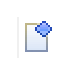
\includegraphics[height=30pt, width=30pt]{../images/usermanual/icon_remote.bmp.eps}
\caption{Local, published \& remote document icons}
\label{default}
\end{center}
\end{figure}

% 3.3.2 USER VIEW
\subsubsection{User View}
\begin{figure}[htbp]
\begin{center}
  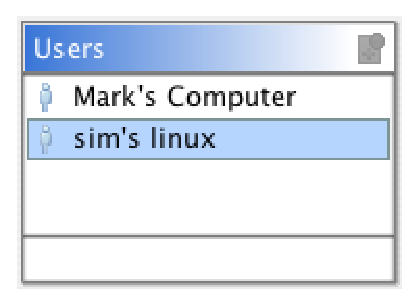
\includegraphics[height=30pt, width=30pt]{../images/usermanual/uview_overview.bmp.eps}
\caption{User View}
\label{default}
\end{center}
\end{figure}

The \textit{User View} shows all other users currently using ACE in your network. This is used to invite (see \ref{Invite / Kick Users}) other users to your published documents. \\
\\
To avoid a complex list with usernames you can use the user view filter. Typing full usernames or parts of it into the textfield below excludes all users not matching.

\begin{figure}[htbp]
\begin{center}
  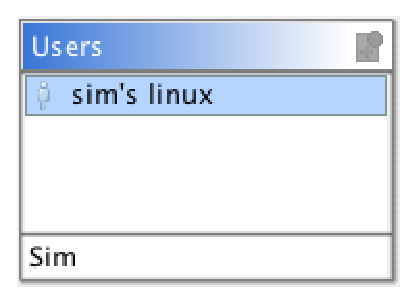
\includegraphics[height=30pt, width=30pt]{../images/usermanual/uview_filtering.bmp.eps}
\caption{User View Filtering}
\label{default}
\end{center}
\end{figure}

% 3.3.3 BROWSE VIEW
\subsubsection{Browse View}

\begin{figure}[htbp]
\begin{center}
  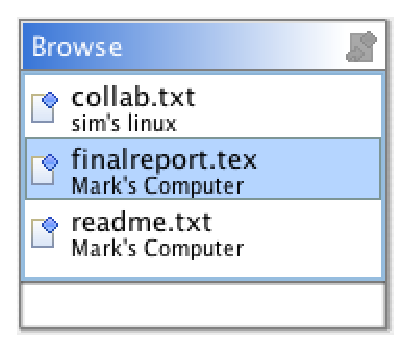
\includegraphics[height=30pt, width=30pt]{../images/usermanual/bview_overview.bmp.eps}
\caption{Browse View}
\label{default}
\end{center}
\end{figure}

The \textit{Browse View} contains a list with all published documents that can be found in a network. Each list entry contains the document title and the name of the publisher. You need this list to join (see \ref{Join / Leave Network Documents}) published documents.

\begin{figure}[htbp]
\begin{center}
  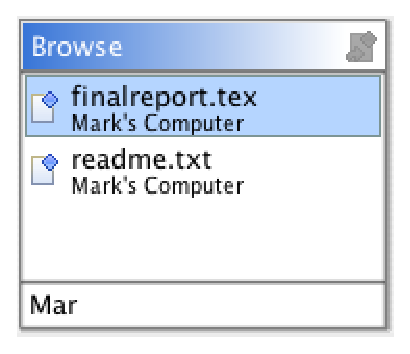
\includegraphics[height=30pt, width=30pt]{../images/usermanual/bview_filtering.bmp.eps}
\caption{Browse View Filtering}
\label{default}
\end{center}
\end{figure}

% 3.3.4 PARTICIPANT VIEW
\subsubsection{Participant View}

\begin{figure}[htbp]
\begin{center}
  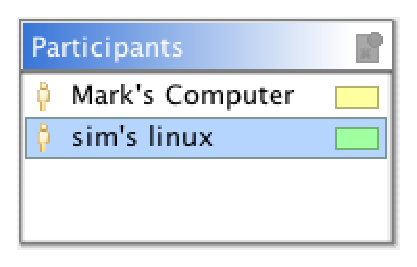
\includegraphics[height=30pt, width=30pt]{../images/usermanual/pview_overview.bmp.eps}
\caption{Participant View}
\label{default}
\end{center}
\end{figure}

When you publish or join a network document you can see a list of all participants in the \textit{Participant View}. Each participant has his own color which is showed on the right side of his username. This colors are used to highlight the text and to draw the cursor or selection from the corresponding participant. If you are the owner of the document you can select a participant and kick (see \ref{Invite / Kick Users}) him from the current document.

% 3.5 PREFERENCES
\subsection{Preferences}






\newpage
% 4. FIRST STEPS
\section{First Steps}

% 4.1 CREATE
\subsection{Create a new Document}

% 4.2 OPEN
\subsection{Open an existing Document}

% 4.3 SAVE
\subsection{Save open Documents}

% 4.4 QUIT
\subsection{Quit}
- save dialogs




\newpage
% 5. NETWORKING
\section{Networking}

% 5.1 PUBLISH / CONCEAL
\subsection{Publish / Conceal Documents}
- (Bild: %editor_view_publish)
- (Bild: %editor_view_conceal)
- (Bild: %nmenu_collaboration_publish)
- (Bild: %nmenu_collaboration_conceal)

% 5.2 INVITE / KICK
\subsection{Invite / Kick Users}
- (Bild: %pview_invite)
- (Bild: %nmenu_collaboration_invite)
- (Bild: %pview_kick)
- (Bild: %nmenu_collaboration_kick)

% 5.3 JOIN / LEAVE
\subsection{Join / Leave Network Documents}
- (Bild: %bview_join.eps)
- (Bild: %dview_joined.eps)

% 5.4 DISCOVER
\subsection{Discover Users}
- (Bild: %nmenu_collaboration_discover)







\end{document}
